%
% File - ch1.tex
%
%
% Description:
% This file should contain the first real chapter or section of your
% thesis.
%
%
%%%%%%%%%%%%%%%%%%%%%%%%%%%%%%%%%%%%%%%%%%%%%%%%%%%%%%%%%%%%%%%%%%%%%%%%%%%%%%%
\section{Exploitation of Quadtree on GPUs}
%%%%%%%%%%%%%%%%%%%%%%%%%%%%%%%%%%%%%%%%%%%%%%%%%%%%%%%%%%%%%%%%%%%%%%%%%%%%%%%

\subsection{CPU Implementation}

The traversal starts from the root node of the quadtree and performs DFS by recursion.
The traversal runs recursively till leaf node is reached. Depth First Search algorithm (DFS) traverses a graph in a depth wise motion and uses recursive function to get the next node to start a search when the bottom of the tree is reached. The traversal starts at the root node and moves down the tree till the bottom of the tree is reached along each branch before backtracking. While visiting each node, it checks for all three conditions to see if a node is completely overlapping,  partially overlapping or not overlapping.

Table~\ref{table:nonlin} illustrates the conditions to satisfy each scenario. N0, N1, N2 and N3 are the four corners of a node and the boundary of the polygon is marked by the four corners, P0, P1, P2, P3  of a rectangle. A checkmark indicates that the corner of the node is within the boundary of all four edges of a polygon. A x mark indicates that the corner of the node is outside the boundary of all four edges of a polygon.
If all the corners of a node is within the four edges of a polygon, then the node is completely overlapping the polygon. If all the corners of a node is outside the four edges of a polygon, then the node is not overlapping the polygon.
If at most three of the corners of a node is outside the four edges of a polygon, then the node is partially overlapping the polygon. All the conditions apart from the ones shown in Table 1 are partially overlapping.

\begin{table}[H]
\centering\begin{tabular}{c c c c c c}
\hline\hline
Case & N0 & N1 & N2 & N3 & Condition \\ [0.5ex] % inserts table 
%heading
\hline
P0 P1 P2 P3 & \checkmark & \checkmark & \checkmark & \checkmark & Completely overlapping \\
P0 P1 P2 P3 & \xmark & \xmark & \xmark & \xmark & Not overlapping \\
\hline
\end{tabular}
\caption{Criteria for Quadtree Node Classification.}
\label{table:nonlin}
\end{table}

Before classifying the node as not overlapping, the polygon is also checked to see if it lies inside the node. If the node is classified as completely overlapping node, then the boundary details of this node is stored and tree is not traversed further from this node. The boundary of the node represents the range of points the node contains and all these points within the node are considered as points within the polygon.
If the node is classified as not overlapping node, then the tree is not traversed further from this node. 
If the node is classified as partially overlapping  node then the tree is traversed further till the leaf node is reached. The points are then extracted from the leaf nodes of the quadtree.

In the case of partially overlapping node, every point needs to be checked to see if it lies within the boundary of the polygon. This check is optimized by classifying the kind of intersection between the node  and the Polygon in such a way that for certain scenarios only either x or y coordinate of the points need to be verified. 

If the intersection of the node is along the horizontal edge of the polygon as in Figure~\ref{fig:overlap2}, then only the y coordinate of the data points inside the node needs to be checked as all the x-coordinate of all points is within the polygon boundary limits. If the intersection between the node and the polygon is along the vertical edge of the polygon as in Figure~\ref{fig:overlap3}, then only the x coordinate of the points needs to be checked as all the y-coordinate of all points is within the polygon boundary limits. For all the other overlap conditions, x-y coordinate of every point is checked with the boundary limits of the polygon.

\begin{figure}[H]
\centering
\vspace{0.5in}
\includegraphics[scale=0.8]{Images/OverlapScenario4}
\vspace{0.5in}
\caption{Overlap of Node on the Horizontal Edge of Polygon.}
\label{fig:overlap2}
\end{figure}

\begin{figure}[H]
\centering
\vspace{0.5in}
\includegraphics[scale=0.8]{Images/OverlapScenario5}
\vspace{0.5in}
\caption{Overlap of Node on the Vertical Edge of Polygon.}
\label{fig:overlap3}
\end{figure}

In the case of GPU implementation, x-y coordinates of all points of the partial node are checked against the polygon edges without classifying them based on the type of node intersection as it will lead to more conditional statements which would increase thread divergence and reduce the performance.

\subsection{GPU Implementation}

Efficient implementation of quadtree traversal in GPU using CUDA is challenging due to the following reasons. 1. The quadtree is an irregular data structure whose memory accesses and work distribution are both irregular and data-dependent. And traversing irregular data structures results in thread divergence.
2. Traversal of a quadtree built using pointers results in lot of pointer-chasing memory operations. Pointer-chasing leads to many un-coalesced memory accesses which affects performance~\cite{barnes:hut}.
3. As done typically the quadtree is built using recursive depth first style in the CPU. Recursive DFS in GPU would be advantageous as it will reduce un-coalesced memory accesses considering the memory for all the structures is preallocated. Recursion can be implemented only on the latest GPUs with CUDA 6.5 version that supports dynamic parallelism, but recursion could lead to low performance due to function call overhead. Recursion on a GPU, requires explicit stack space per thread and deep recursion will cause overflow of the available stack space and in this case CUDA may reduce the maximum physical threads per launch.
4. Transferring a pointer based quadtree to a GPU proves to be a challenge. Though this task can be implemented with "cudamallocamanaged" function, debugging becomes harder.

To take advantage of the parallel nature of the GPUs, BFS is used instead of DFS. 
The quadtree is queried to find the points inside a polygon by first finding the quadtree nodes that overlap the polygon. Once the nodes that overlap the polygon are determined, the points inside the polygon can be found from these nodes. Given a set of nodes, arranged hierarchically, the system needs to find the minimum set which solves the query correctly. This can be done by assigning one thread to a polygon but there is not enough stack space. Since our GPU implementation method requires an explicit array in the shared memory for each polygon, assigning one thread to a polygon will also pose a limit on the number of polygons processed simultaneously by a block due to the limitation in the shared memory size.
The stack space per thread needs to be reduced and optimization for thread divergence and memory access should be done. To minimize thread divergence and reduce stack space per thread and also achieve maximum parallelization, a polygon is assigned to a warp instead of a thread or a block of threads. To optimize for memory access, memory preallocation for the input points, query polygons, point buffer (list that holds points within a leaf node of quadtree) is done on the CPU.

CUDA applications exploit massive data parallelism and it is capable of processing massive amount of data within a short period of time. But data accesses to GDDR DRAM global memory limits this performance due to limitations in global memory bandwidth. Therefore algorithms and techniques need to be employed in order to reduce the demand on the DRAM bandwidth  and make efficient use of the data accessed from the global memory~\cite{Kirk:2010:PMP:1841511}.


The quadtree is built on the CPU from heap objects and each heap object has several fields. For example, each quadtree node object contains 4 child pointers and  data fields which stores the attributes of the node. Other heap objects include data points and point buffers. 
Though the CPU implementation benefits from the dynamic memory allocation, the use of the C library malloc is not preferred for the CPU-GPU implementation because this dynamic memory-management function provides allocation and de-allocation of arbitrary segments of memory. In order to improve performance on the GPU, the access to memory segments need to be coalesced. The memory preallocation places the consecutive points and point buffers sequentially in memory and therefore results in memory coalesced access as the points close to one other are more likely to be within the same polygon boundary. But preallocating memory for the  quadtree nodes is not expected to improve performance as the nodes are stored in a depth first fashion in the CPU but a BFS traversal is done on the GPU.

The DRAM cores are slower as the market demands a high capacity rather than a lower latency DRAM.  These cores operate at much lower speed compared to the interface speed. GDDR4 operates at 1/8th of the interface speed and this difference will increase with every generation of GDDR as the storage capacity increases~\cite{Kirk:2010:PMP:1841511}.
Since DRAM cores are slower than the interface, the system needs to increase the buffer width to feed into faster interface. The modern DRAM banks are designed to be accessed in burst mode. If the accesses are not to sequential locations, the transferred burst bytes are discarded.
In order to take full advantage of the DRAM system in CUDA environment, the system needs to make sure that the processor makes use of all the data bursted out of the DRAM chip.
Thus from a memory throughput standpoint to get peak memory performance, computation must be structured around sequential memory accesses~\cite{Kirk:2010:PMP:1841511}. Random memory access leads to a huge performance penalty due to random memory reads.


\subsubsection{Drawbacks on implementing DFS on GPU}

One option to traverse down the tree for every polygon is to use DFS by assigning a warp or a thread to each polygon. But the DFS implementation in the GPU would cause a overhead due to the data movement as the thread moves up and down the tree. In this case the interior nodes of the tree are repeatedly visited as a thread has to return to higher level of the tree to traverse down to other children~\cite{goldfarb13sc}. This results in additional work for each thread.

\subsubsection{BFS Implementation on GPU}


Stack based breadth first tree-traversal allows parallelization. To take advantage of the parallel nature of the GPU, the threads are launched at level 3 of the quadtree instead of the root node. Starting at the root node will result in only one thread being active for level 1 traversal of quadtree. Starting at a deeper level prevents this and results in more parallelism.
Initially the index of the node from level 3 of the quadtree is stored in an array in the shared memory.
This index is used to fetch the quadtree node from the global memory.

Here the tree is traversed down to find the boundaries of a polygon and thus extracting the quadtree nodes within that boundary or partially overlapping the boundary. For completely overlapping nodes, the boundary of the node gives the range of points within the polygon. This method is more efficient than traversing down the quadtree to find the individual points within the polygon in terms of computation and also memory. And for partially overlapping nodes, each point needs to be checked against the boundary of the polygon. With this information, the range of points within the polygon region can be found and this range is stored instead of individual points to save memory on the GPU. If there are a very large number of input points and query polygons, then storing individual points for each polygon will result in overflow of the memory. 

The Polygons are associated with a CUDA warp, where the number of threads in a warp depends on CUDA configuration. By launching thousands of GPU blocks in parallel, 'N' number of polygons can be queried, where N = (size of each block / 32)*(total number of blocks).  Each warp executes the same algorithm but on a different polygon. Assigning a warp to a polygon will result in less thread divergence. Each thread in a warp reads x, y co-ordinate of all four corners of a polygon which is required for the tree traversal.

The GPU kernel replaces the recursive call with stack push operations that save indices of each child of a node traversed, that satisfies the query. Traversal is facilitated by a loop that simultaneously assigns the indices of the nodes in the stack to threads in warp until the stack is empty, indicating there are no more nodes to visit at that level for a polygon. To save stack space, node indices are stored in the stack instead of the node. At the beginning of each iteration of the loop the nodes are popped from the stack. After popping the node from the stack, the function which checks for the overlapping conditions is executed on that node, possibly pushing more nodes onto the stack or returning when it reaches a node that fails the criteria, an empty node or a leaf node.

If the number of nodes in the stack exceeds the number of threads assigned to a polygon, then loop over with increments of the number of threads in a warp is done. Within each loop, each node is assigned to one thread.
Each thread reads the quadtree node's properties and tests whether or not to traverse the tree further down from this node. If the criteria to traverse the tree down from this node is satisfied, then the indices of the node's all four children is added to the stack, provided the child is not an empty node. One stack space is assigned to each polygon. Traversal at each level of quadtree is synchronized, so that the same stack can be re-used for a polygon. The tree-traverse loop is repeated until all the levels of the quadtree is visited.
The number of GPU threads used per level is equal to the number of nodes that was pushed on to the stack from the previous iteration.

The warp starts the traversal at level 3 of the quadtree. The indices of children of the nodes that satisfy the query are placed in an array. The condition checks whether a node is overlapping the polygon. Once the indices of children of the nodes that satisfy the query are placed in an array and the other nodes, which do not satisfy the condition are ignored, the next level is evaluated.
Once the leaf node is reached, the nodes are classified as completely and partially overlapping nodes. And from these nodes all the points that are inside the Polygon are taken. The boundaries of the completely overlapping nodes which give the range of points within the nodes are stored.

In the case of partially overlapping nodes, each point within the node is checked against the boundary of the polygon and the range of points that lie within the polygon is stored. At the last level of the tree, the warp still holds the polygon and the threads within a warp is assigned to a leaf node that is either partially or completely overlapping the polygon. Each of these threads compute the points within each node that are inside the polygon.

This approach will minimize the use of shared memory space, as only the indices of nodes are stored starting from level 3 in shared memory instead of the node itself that satisfy the required criteria. The indices of the nodes are used to fetch the corresponding node from the global memory.
The order in which the nodes are stored in the stack does not matter, as every level in the quadtree is processed independent of the previous and every node is processed independent of other nodes in the stack.

The indices of the nodes are saved in the stack array in the shared memory and the the stack is cleared after computing every level. Shared memory blocks are used in order to gain significant speedups of approximately 150 to 200 times~\cite{Kelly:gpu}. If a node index returns -1, then the node is empty and it is not fetched from the global memory.
The number of nodes that needs to be visited  at the next level is also stored in a shared memory variable for every polygon and it is incremented atomically. The iterative loop launches threads based on the count on this variable. The loop executes till the last level of quadtree is reached.

To implement this algorithm, the maximum number of levels in a quadtree should be 4 because of the limitations in the size and the number of stacks in the  shared memory. As the number of levels in a quadtree increases, the maximum stack space required per polygon would also increase and this will limit the number of polygons processed.

The size of shared memory per block on the GTX680 is 49152 bytes~\cite{nvidia:12:gtx680tech}. As there are 32 warps in a block by default, each block is assigned  32 polygons. Each polygon requires an array in the shared memory in order to store the node indices from each level that needs to be further traversed. The maximum array size required for a 4 level quadtree is 64 as the maximum number of nodes at the leaf is 64. This allocation occupies a shared memory space of 32 * 64 *4 = 8192 bytes, which is well within the limit. The array size for each polygon needs to be increased to 256 for a 5 level quadtree. This allocation results in a shared memory usage of 256 * 32 * 4  = 66560 bytes, which exceeds the available shared memory size. Therefore unless a larger size of shared memory becomes available in the future, the quadtree cannot not be subdivided beyond level 4 in this case.

In Figure~\ref{fig:bfs_gpu}, the check mark indicates that the node  satisfies the query and the tree will be further traversed from this node. The cross mark indicates either that the node does not satisfy the query or the node is empty and the threads terminate at this point without proceeding further.

\begin{figure}[H]
\vspace{0.5in}
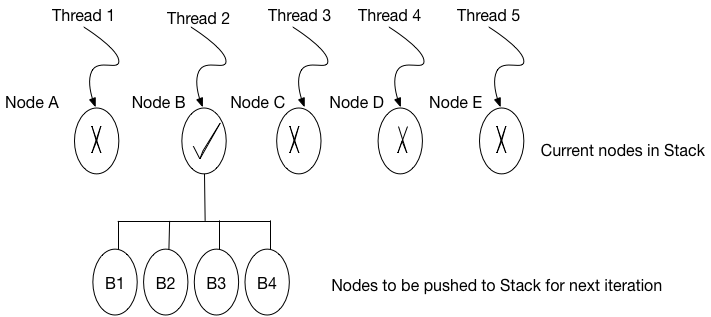
\includegraphics[scale=0.5]{Images/BFSgpu}
\vspace{0.5in}
\caption{BFS GPU Implementation.}
\label{fig:bfs_gpu}
\end{figure}

The traversal starts at level 3 of the quadtree. The children of the nodes that satisfy the overlap conditions are pushed in to the array. The array is initialized after every iteration. 
The cross mark indicates that the node is either not satisfying the overlap conditions or it is empty. The nodes are stored in the array in any order. The process repeats till bottom of the tree is reached. 
The number of stack array in the shared memory per block depends on the number of warps in a block. At the most, the iterative loop processes 32 nodes at a time by default (equal to the number of threads in a warp). The conditional statements are changed to avoid function return statements to prevent the traversal loop from prematurely exiting and preventing the remainder of the loop body from executing.

A polygon is checked against the node of the quadtree for 3 scenarios such as, completely overlapping,  partially overlapping and not overlapping.
All nodes are checked for "not overlapping" conditions till leaf node is reached. If a node satisfies the condition then the tree is not traversed from this node and if the node does not satisfy the condition, then its children are placed in the stack and the traversal continues.

The number of checks for a partially overlapping node is more and use of "if" statements decreases the performance due to control divergence. If threads within a warp take different paths, then 2 passes on the different path of the code is required to execute all threads. Since different execution paths are serialized, it leads to performance penalty.

Therefore in order to reduce conditional statements (if statements), the condition for completely overlapping node is first computed on the leaf nodes and the nodes that satisfies the condition is classified as completely overlapping nodes and nodes that does not satisfy the condition is classified as partially overlapping nodes. The Figure~\ref{fig:FlowChart}, shows the high level overview of the algorithm to find the points in polygon using quadtree on a GPU. 

\begin{figure}[H]
\centering
\vspace{0.5in}
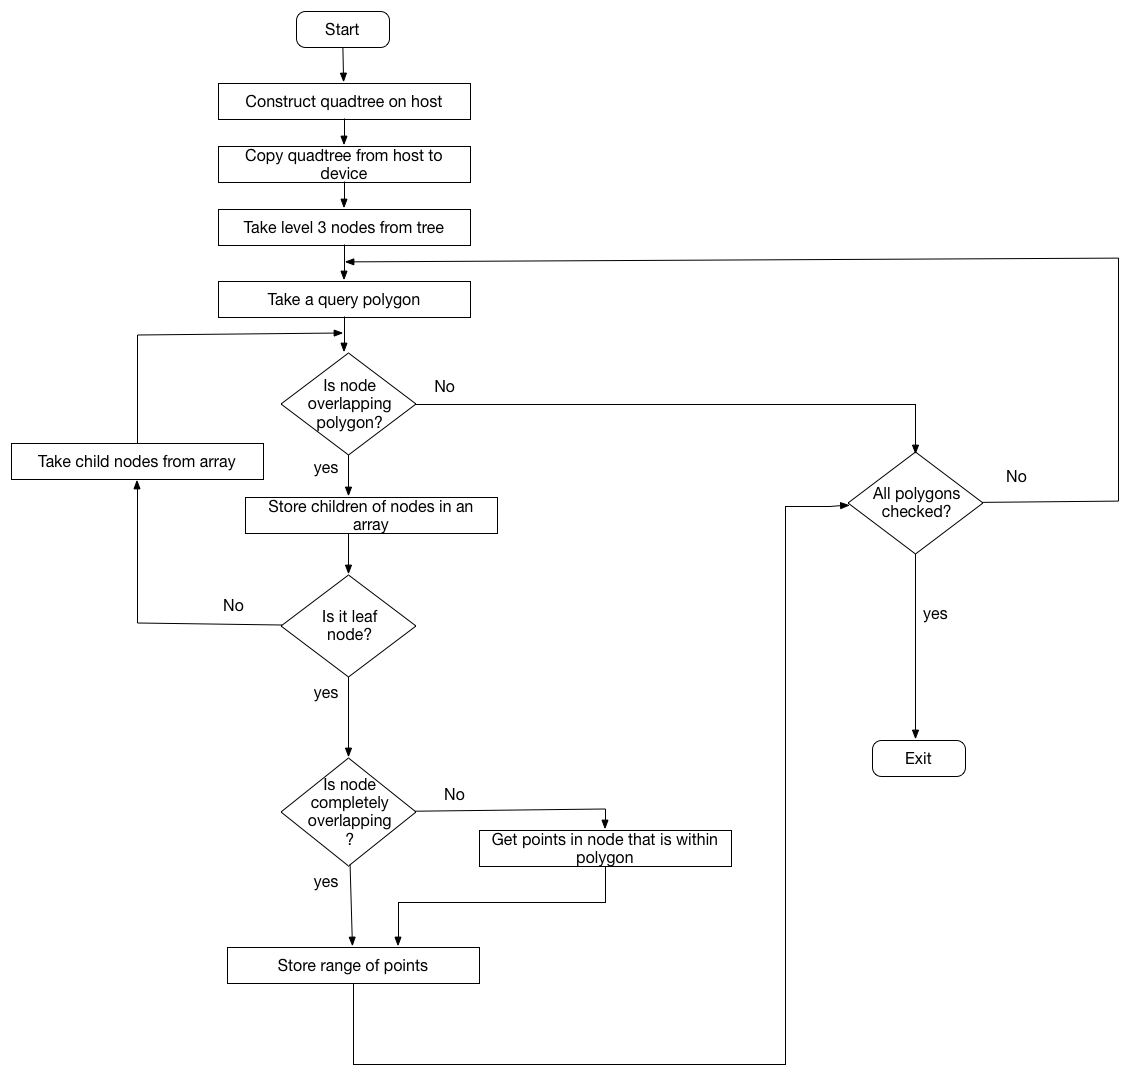
\includegraphics[scale=0.35]{Images/FlowChart}
\vspace{0.5in}
\caption{Process Flow.}
\label{fig:FlowChart}
\end{figure}

\subsection{BFS Implementation on GPU - Different Scenarios of Query Polygon}

The Figure~\ref{fig:level1quadtree}, Figure~\ref{fig:level2quadtree}, Figure~\ref{fig:level3quadtree} and Figure~\ref{fig:level4quadtree} show the data points (left)  and its corresponding tree representation (right). These data points will be analyzed for different polygon overlap scenarios in the next sections.
The numbers inside the circle represent the index of the node at that level.
Figure~\ref{fig:level1quadtree} shows the root node that contains all input data points. The root node is subdivided into 4 equal regions to form 4 nodes at level 2.
Figure~\ref{fig:level2quadtree} shows the four children of the root node. Root node has all four children as the data points are present in all four directions (NW, NE, SW, SE) of the root node. The nodes at level 2 are again subdivided equally to form the child nodes.
Figure~\ref{fig:level3quadtree}, shows the nodes at level 3 of the quadtree. Child node 3 of parent node 1 from level 2, child node 1 and child node 4 of parent node 3 from level 2 and child node 3 of parent node 4 from level 2 are empty as the parent nodes did not have any points in those directions.
Figure~\ref{fig:level4quadtree} shows the child nodes at level 4. Many of the nodes at this level are empty as they do not contain any points.


\begin{figure}[H]
  \centering
  \vspace{0.5in}
  \begin{minipage}[b]{0.35\textwidth}
    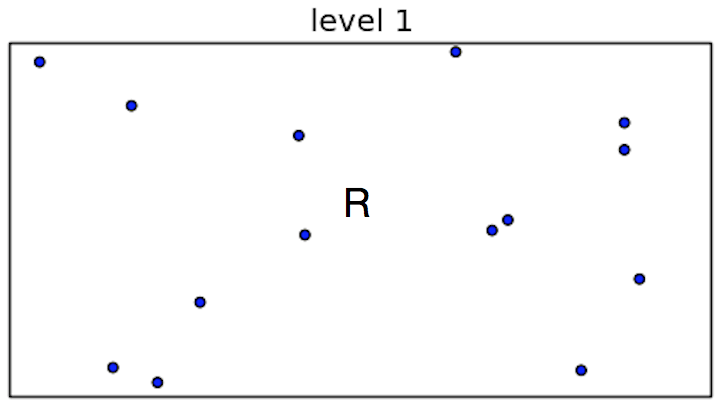
\includegraphics[width=\textwidth]{Images/Quadtree_basic_scenario6}
  \end{minipage}
  \hfill
  \begin{minipage}[b]{0.4\textwidth}
    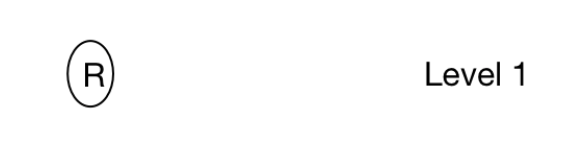
\includegraphics[width=\textwidth]{Images/R1}
  \end{minipage}
  \vspace{0.5in}
  \caption{Level 1 Quadtree.}
  \label{fig:level1quadtree}
\end{figure}

\begin{figure}[H]
  \centering
  \vspace{0.5in}
  \begin{minipage}[b]{0.35\textwidth}
    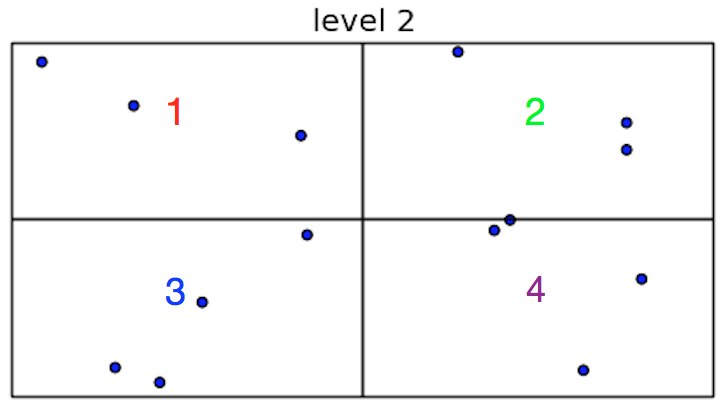
\includegraphics[width=\textwidth]{Images/Quadtree_basic_scenario7}
  \end{minipage}
  \hfill
  \begin{minipage}[b]{0.6\textwidth}
    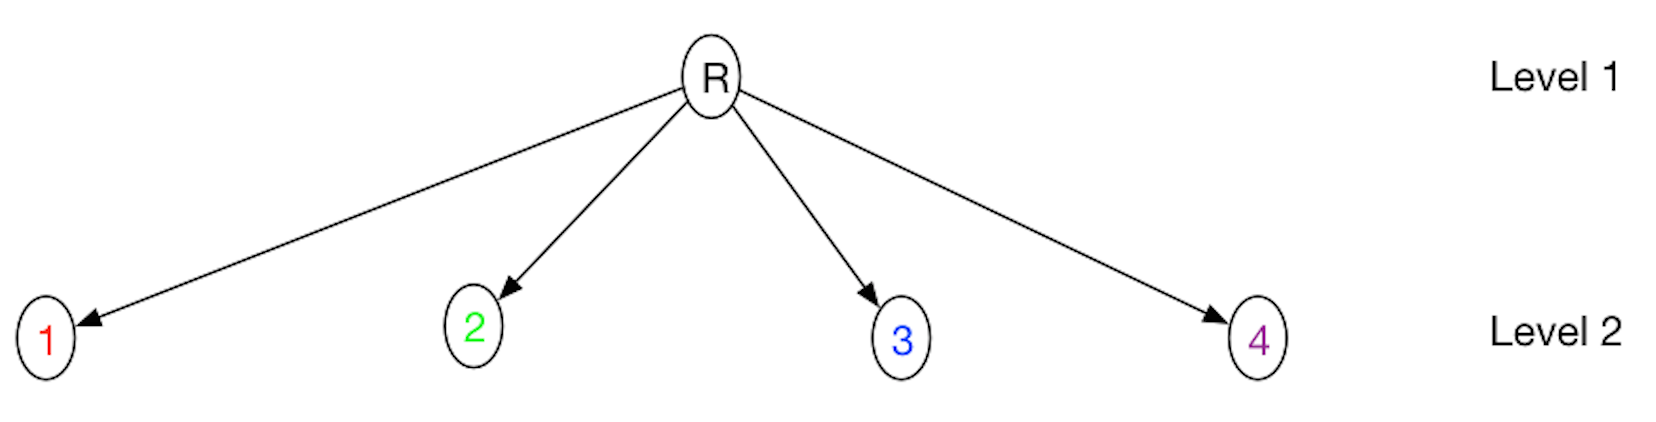
\includegraphics[width=\textwidth]{Images/L2_Tree}
  \end{minipage}
  \vspace{0.5in}
  \caption{Level 2 Quadtree.}
  \label{fig:level2quadtree}
\end{figure}

\begin{figure}[H]
  \centering
  \vspace{0.5in}
  \begin{minipage}[b]{0.35\textwidth}
    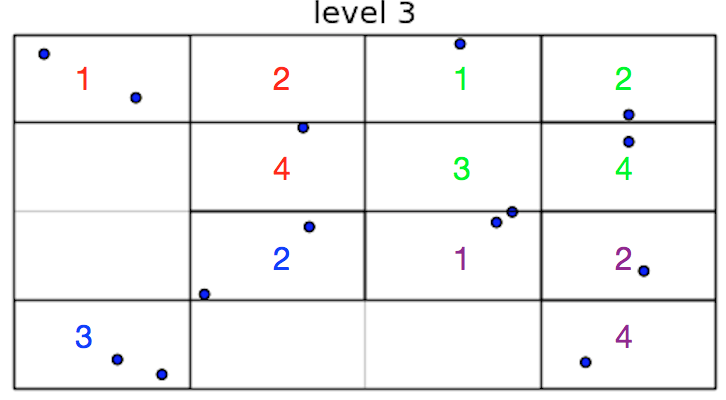
\includegraphics[width=\textwidth]{Images/Quadtree_basic_scenario8}
  \end{minipage}
  \hfill
  \begin{minipage}[b]{0.6\textwidth}
    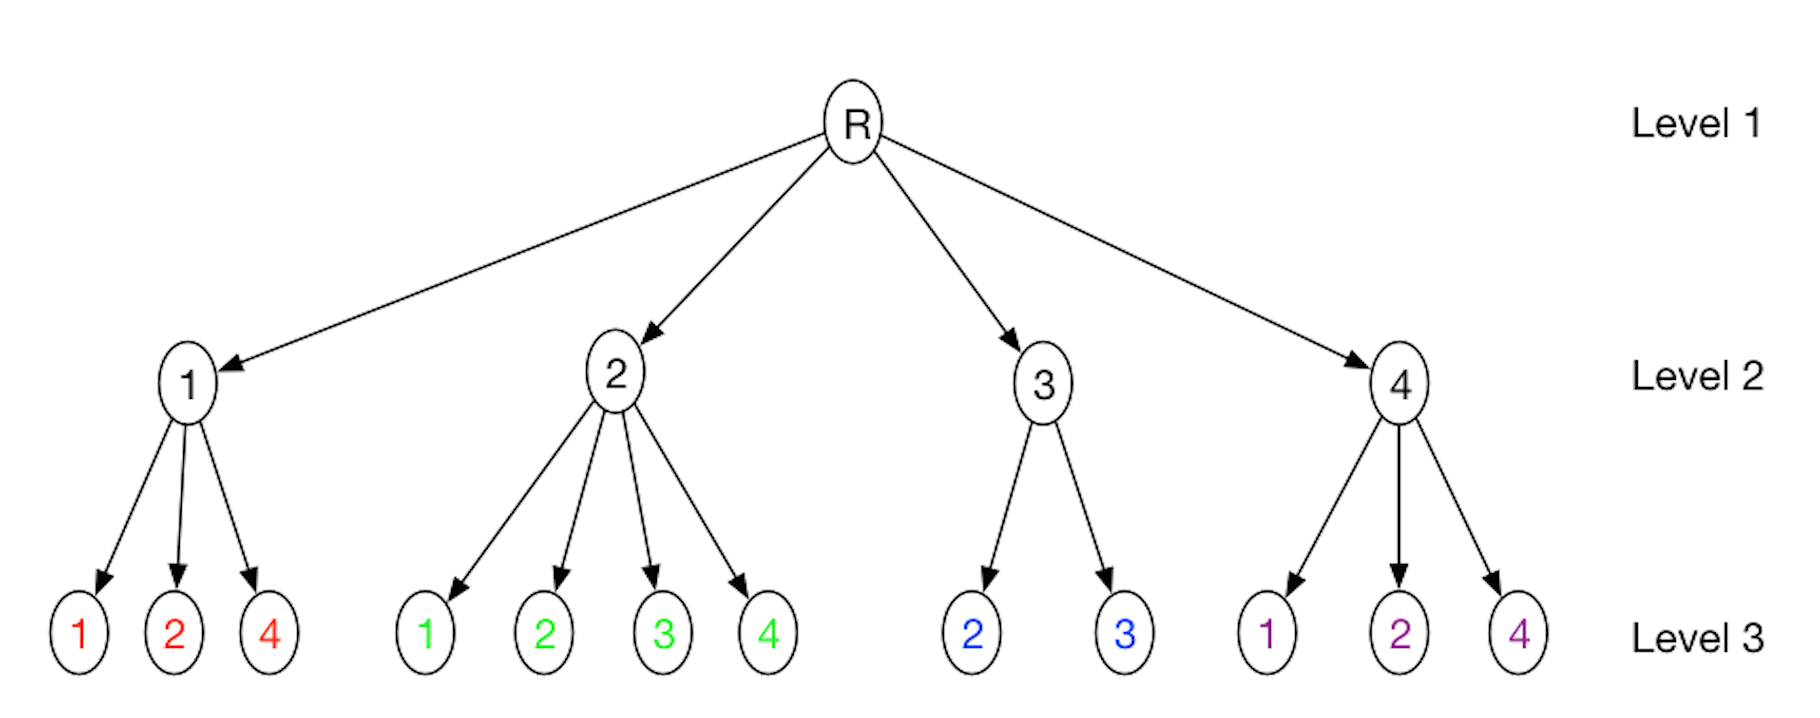
\includegraphics[width=\textwidth]{Images/L3_Tree}
  \end{minipage}
  \vspace{0.5in}
  \caption{Level 3 Quadtree.}
  \label{fig:level3quadtree}
\end{figure}

\begin{figure}[H]
  \centering
  \vspace{0.5in}
  \begin{minipage}[b]{0.35\textwidth}
    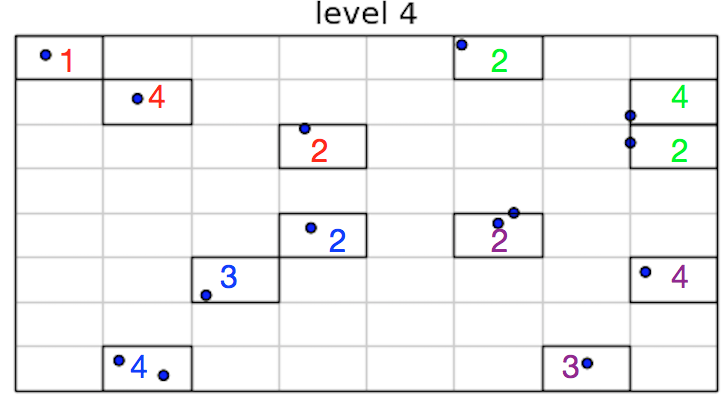
\includegraphics[width=\textwidth]{Images/Quadtree_basic_scenario9}
  \end{minipage}
  \hfill
  \begin{minipage}[b]{0.6\textwidth}
    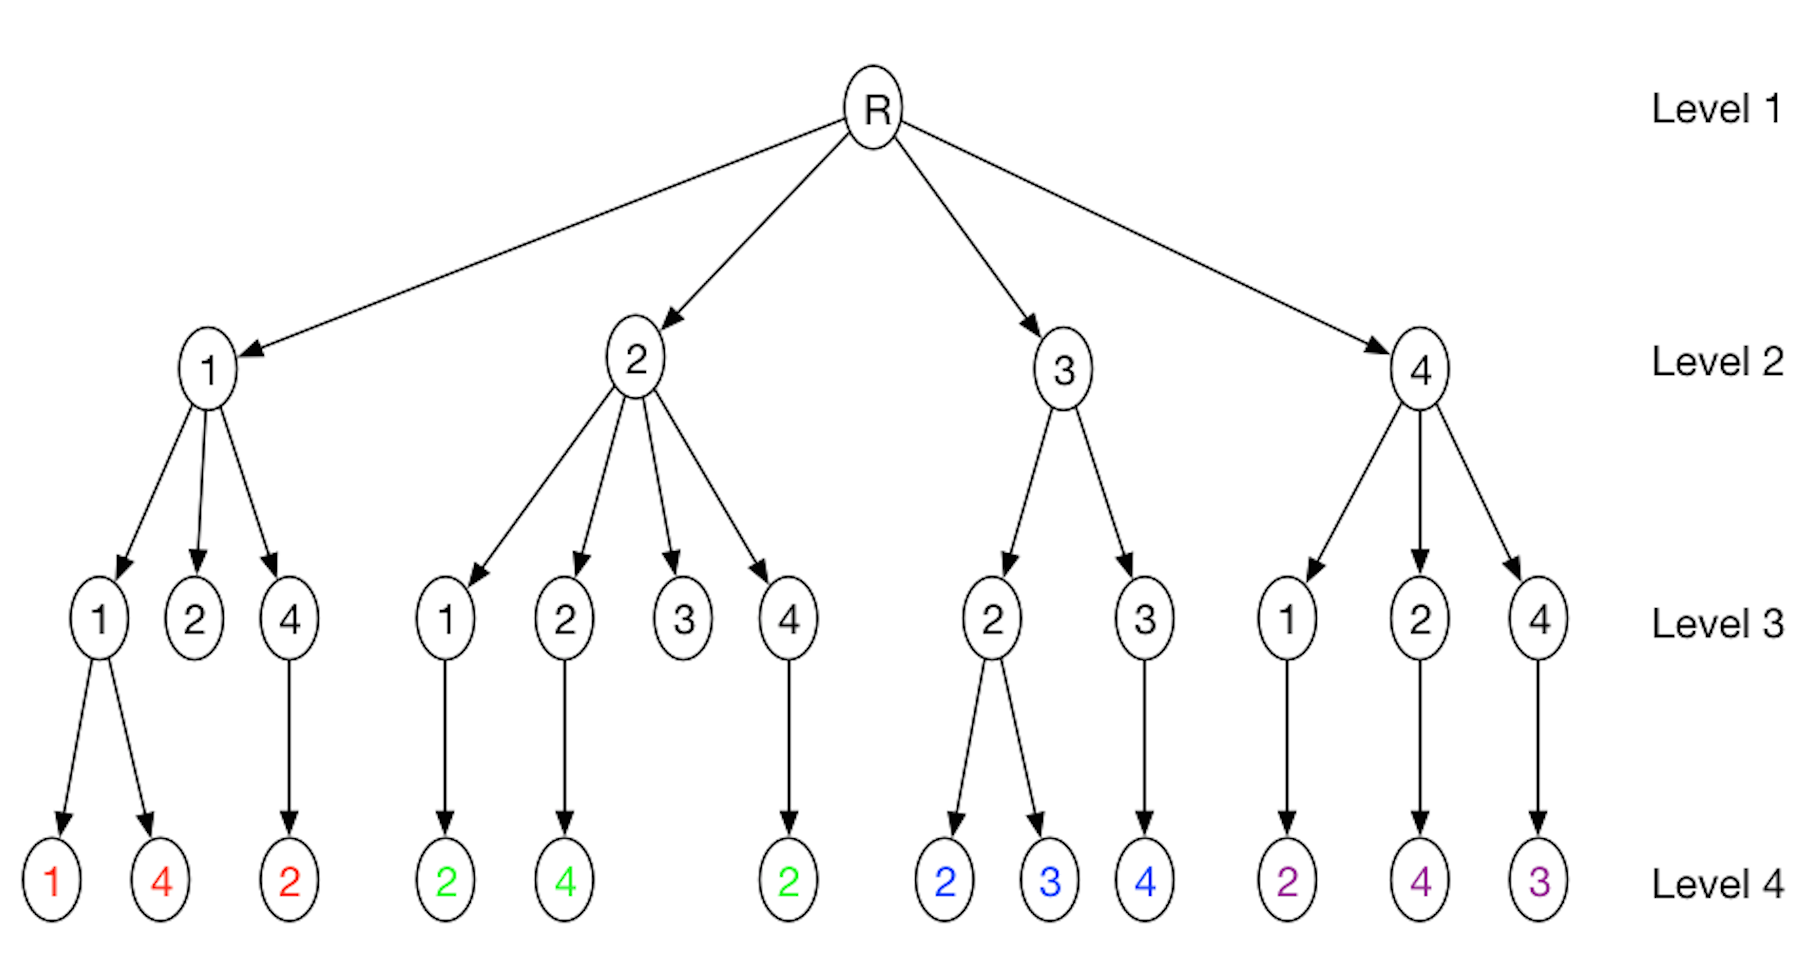
\includegraphics[width=\textwidth]{Images/L4_Tree}
  \end{minipage}
  \vspace{0.5in}
   \caption{Level 4 Quadtree.}
  \label{fig:level4quadtree}
\end{figure}

\clearpage
\subsubsection{Query Polygon inside a Leaf Node}

Figure~\ref{fig:Level1} shows the first scenario that demonstrates the best case scenario where the polygon lies within one quadrant at level 4 of the quadtree and the algorithm provides best performance.

\begin{figure}[H]
  \centering
  \vspace{0.5in}
  \begin{minipage}[b]{0.35\textwidth}
    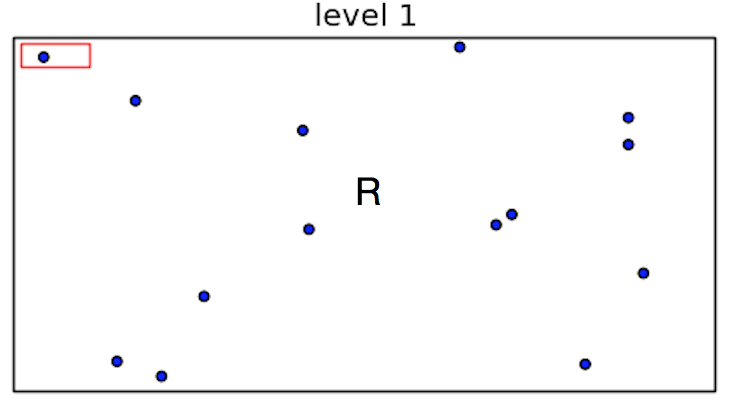
\includegraphics[width=\textwidth]{Images/1_1Quad1_1}
  \end{minipage}
  \hfill
  \begin{minipage}[b]{0.5\textwidth}
    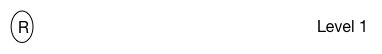
\includegraphics[width=\textwidth]{Images/1_1Quad_1_tree}
  \end{minipage}
  \vspace{0.5in}
   \caption{Sample Datapoints (left) and the Quadtree (right) at Level 1.}
   \label{fig:Level1}
\end{figure}


Figure~\ref{fig:Level2} shows that at level 2, the algorithm isolates one quadrant (first child of the root node) and ignores all other quadrants, thus bringing down the number of quadrants to be processed to 1 from 4 (4 is the total number of nodes at this level).

\begin{figure}[H]
  \centering
  \vspace{0.5in}
  \begin{minipage}[b]{0.35\textwidth}
    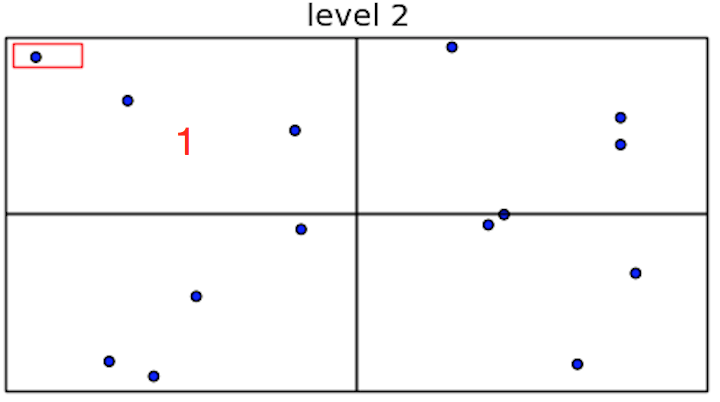
\includegraphics[width=\textwidth]{Images/1_1Quad1_2}
  \end{minipage}
  \hfill
  \begin{minipage}[b]{0.5\textwidth}
    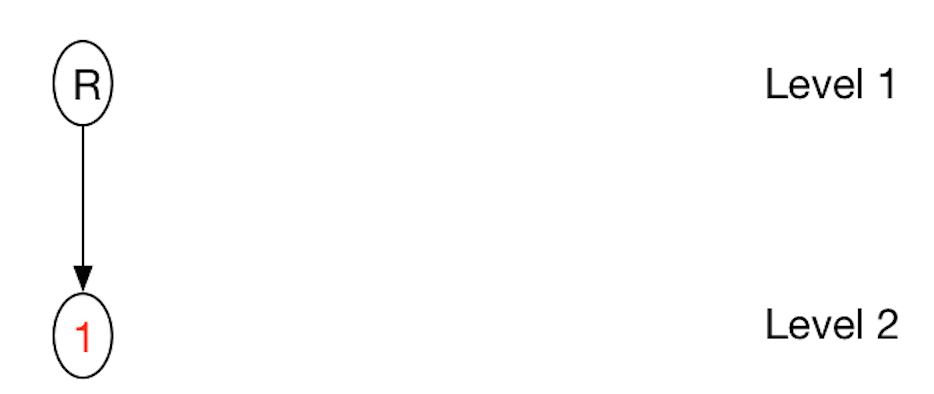
\includegraphics[width=\textwidth]{Images/1Quad_2_tree}
  \end{minipage}
  \vspace{0.5in}
  \caption{Sample Datapoints (left) and the Quadtree (right) at Level 2.}
   \label{fig:Level2}
\end{figure}

Figure~\ref{fig:Level3} shows that at level 3, the algorithm again isolates one quadrant which is the first child of the quadrant from level 1. This step reduces the number of quadrants to be processed to 1 from 3 (3 is the total number of children of the node output from level 1).

\begin{figure}[H]
  \centering
  \vspace{0.5in}
  \begin{minipage}[b]{0.35\textwidth}
    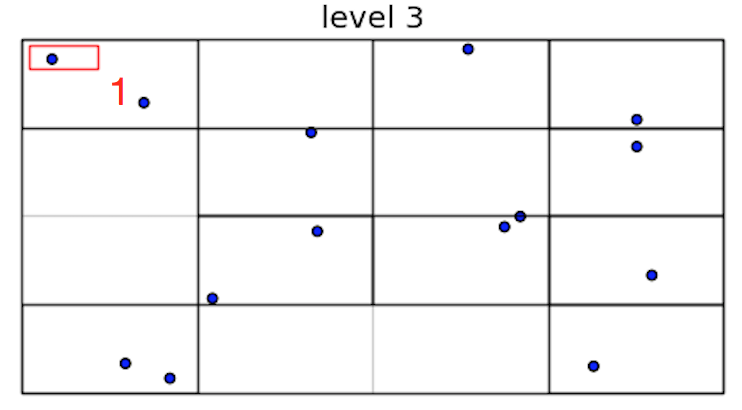
\includegraphics[width=\textwidth]{Images/1_1Quad1_3}
  \end{minipage}
  \hfill
  \begin{minipage}[b]{0.5\textwidth}
    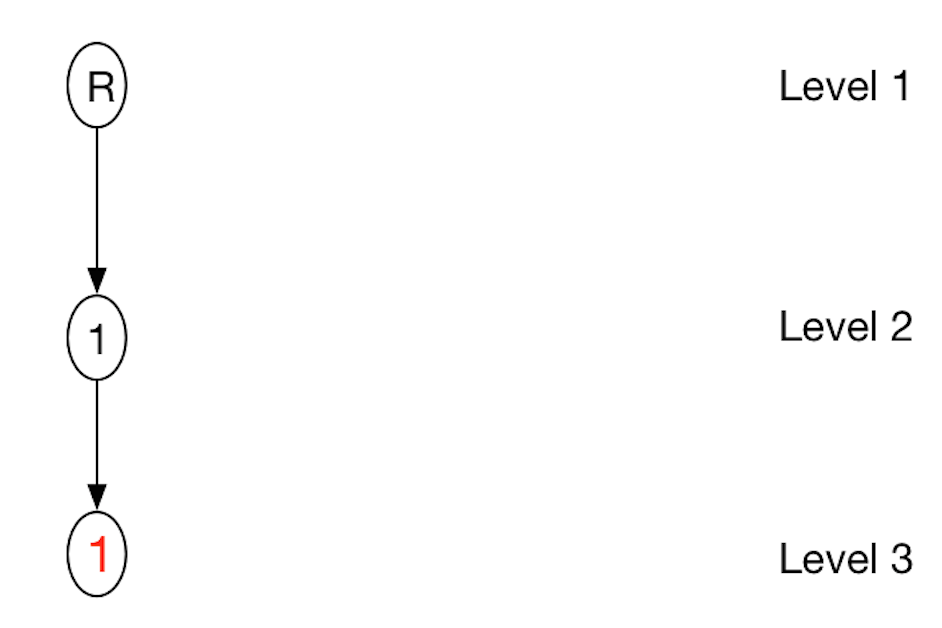
\includegraphics[width=\textwidth]{Images/1Quad_3_tree}
  \end{minipage}
  \vspace{0.5in}
\caption{Sample Datapoints (left) and the Quadtree (right) at Level 3.}
   \label{fig:Level3}
\end{figure}


In Figure~\ref{fig:Level4} at level 4, the algorithm isolates one quadrant which is the first child of the quadrant from level 3. This step reduces the number of quadrants to be processed to 1 from 2 (2 is the total number of children of the node output from level 3).
Finally only one quadrant at level 4 needs to be processed in order to get the points inside the polygon in this case.

\begin{figure}[H]
  \centering
  \vspace{0.5in}
  \begin{minipage}[b]{0.35\textwidth}
    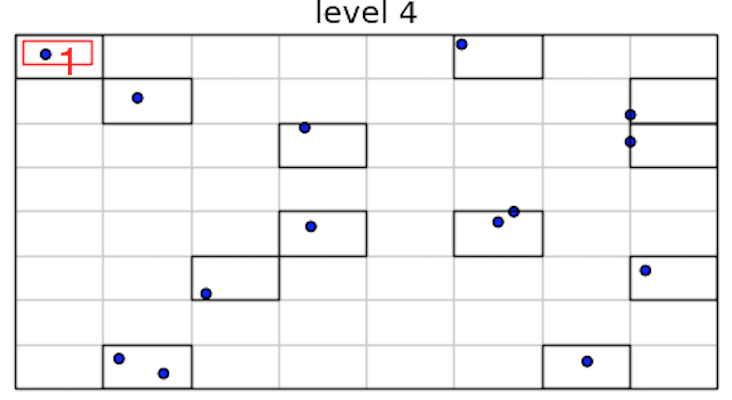
\includegraphics[width=\textwidth]{Images/1_1Quad1_4}
  \end{minipage}
  \hfill
  \begin{minipage}[b]{0.5\textwidth}
    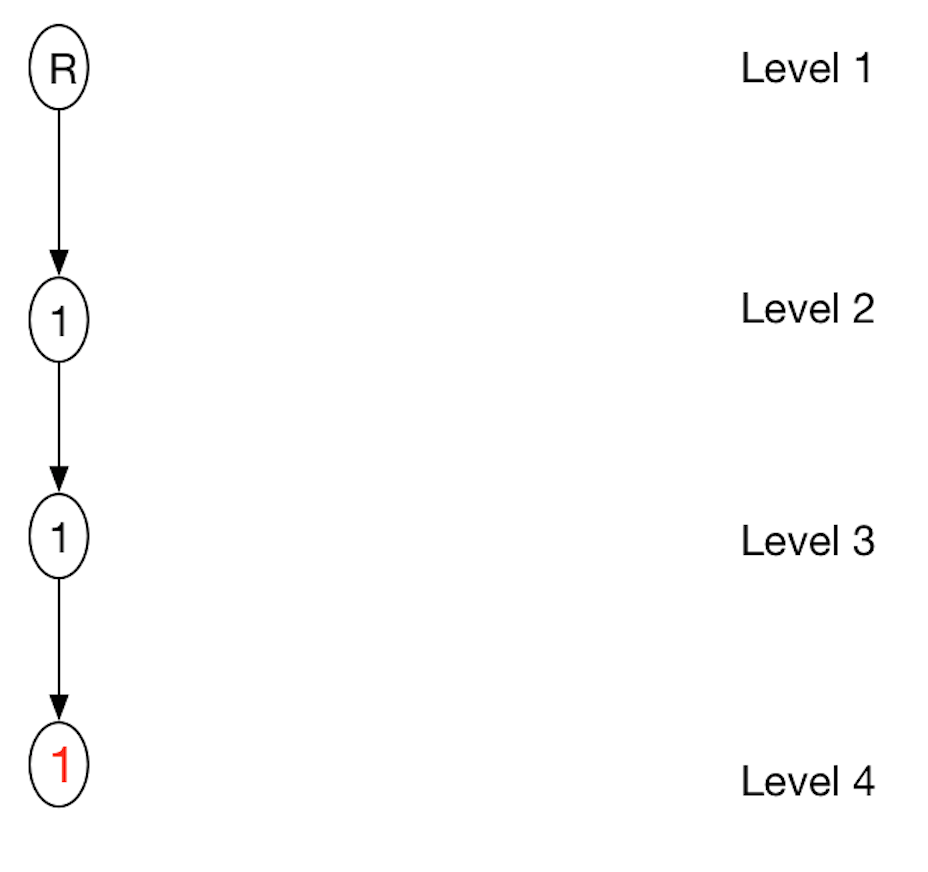
\includegraphics[width=\textwidth]{Images/1Quad_4_tree}
  \end{minipage}
  \vspace{0.5in}
  \caption{Sample Datapoints (left) and the Quadtree (right) at Level 4.}
  \label{fig:Level4}
\end{figure}

\subsubsection{Polygon overlapping 2 nodes}

Figure~\ref{fig:quad_1_1} shows the second scenario that demonstrates a condition where the query polygon overlaps 2 nodes at level 2 and the algorithm provides a medium performance. 

\begin{figure}[H]
  \centering
  \vspace{0.5in}
  \begin{minipage}[b]{0.35\textwidth}
    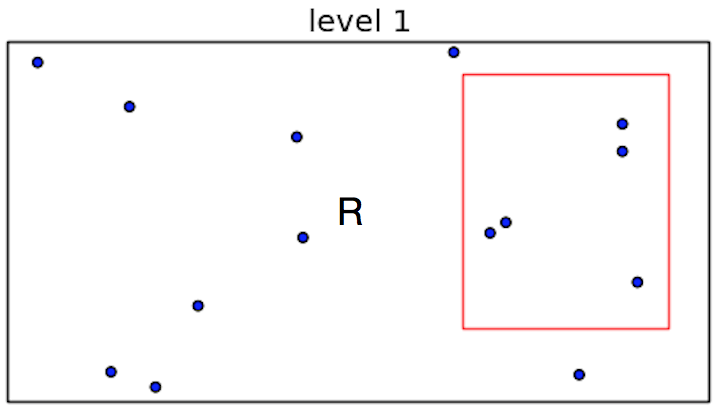
\includegraphics[width=\textwidth]{Images/2Quad_1}
  \end{minipage}
  \hfill
  \begin{minipage}[b]{0.6\textwidth}
    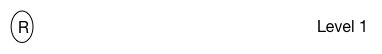
\includegraphics[width=\textwidth]{Images/1_1Quad_1_tree}
  \end{minipage}
  \vspace{0.5in}
  \caption{Sample Datapoints (left) and the Quadtree (right) at Level 1.}
  \label{fig:quad_1_1}
\end{figure}

Figure~\ref{fig:quad_2_2} shows that at level 2, the algorithm isolates two quadrants (second and fourth child of the root node) and ignores the other two quadrants, thus bringing down the number of quadrants to be processed to 2.


\begin{figure}[H]
  \centering
  \vspace{0.5in}
  \begin{minipage}[b]{0.35\textwidth}
    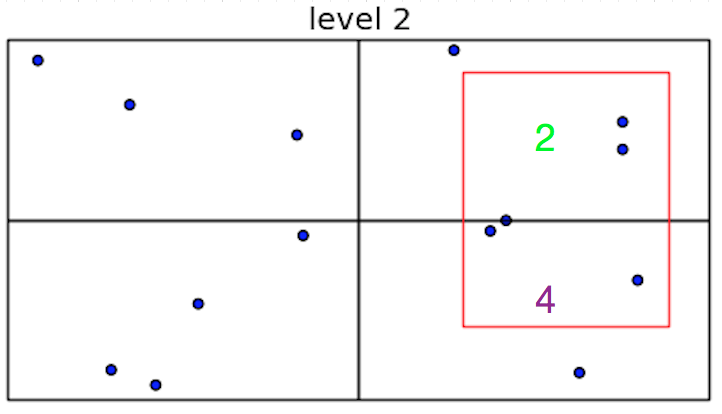
\includegraphics[width=\textwidth]{Images/2Quad_2}
  \end{minipage}
  \hfill
  \begin{minipage}[b]{0.6\textwidth}
    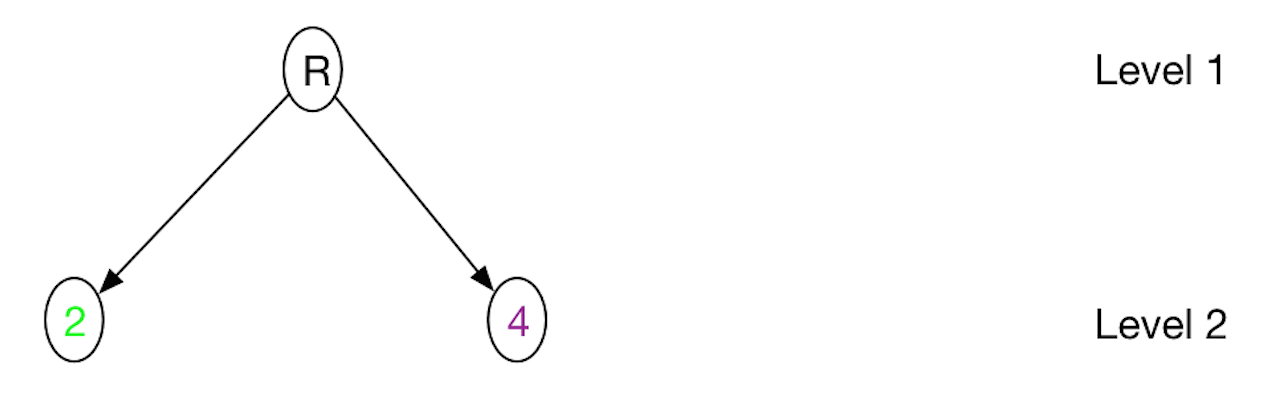
\includegraphics[width=\textwidth]{Images/2Quad_2_tree}
  \end{minipage}
  \vspace{0.5in}
  \caption{Sample Datapoints (left) and the Quadtree (right) at Level 2.}
   \label{fig:quad_2_2}
\end{figure}

Figure~\ref{fig:quad_2_3} shows that level 3, the algorithm isolates 7 quadrants which are the all four children of the second child of root node and first, second and fourth child of the fourth child of root node.
This step reduces the number of nodes to be processed by one as one of the child of the nodes output from the previous level is empty.

\begin{figure}[H]
  \centering
  \vspace{0.5in}
  \begin{minipage}[b]{0.35\textwidth}
    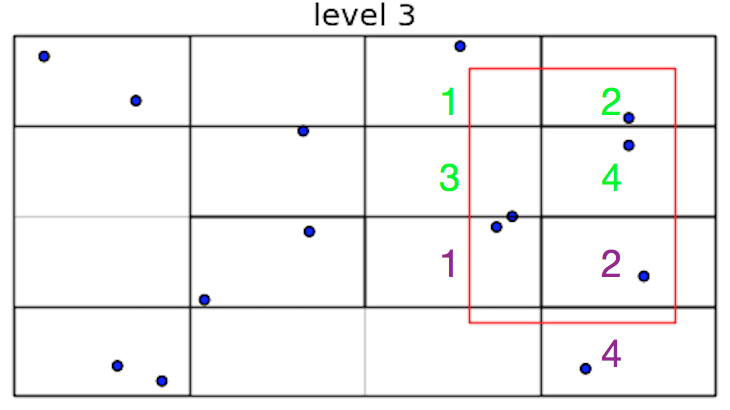
\includegraphics[width=\textwidth]{Images/2Quad_3}
  \end{minipage}
  \hfill
  \begin{minipage}[b]{0.6\textwidth}
    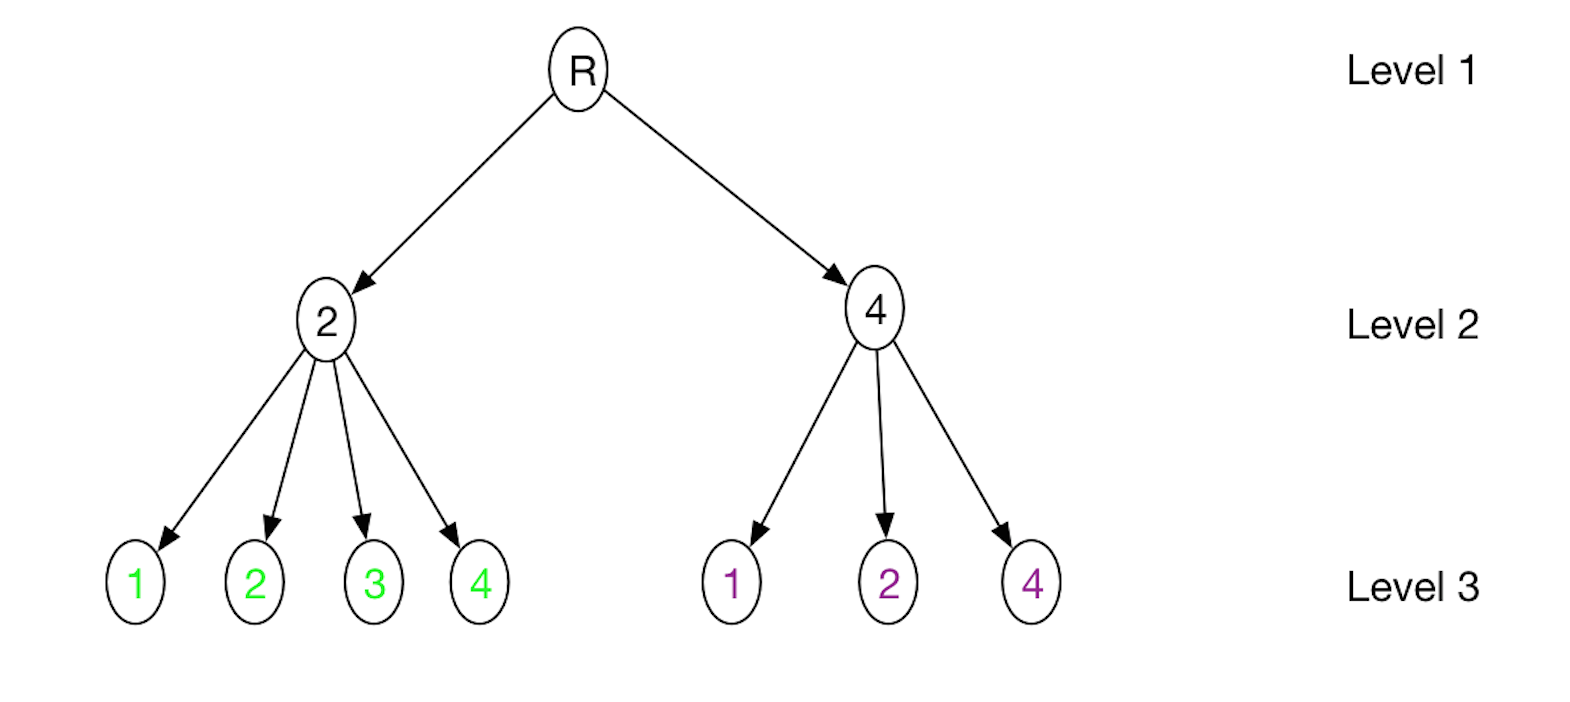
\includegraphics[width=\textwidth]{Images/2Quad_3_tree}
  \end{minipage}
  \vspace{0.5in}
  \caption{Sample Datapoints (left) and the Quadtree (right) at Level 3.}
  \label{fig:quad_2_3}
\end{figure}

Figure~\ref{fig:quad_2_4} shows that at level 4, the algorithm isolates 5 quadrants from the children of 7 quadrants from previous level. By traversing down to level 4, the number of data points that need to be evaluated are reduced by ignoring 3rd child of the 4th child from level 3. If the quadrant that is ignored at level 4 has a larger number of data points, then using a 3-level quadtree would have resulted in a huge performance penalty.
Finally only 5 quadrants at level 4 needs to be processed in order to get the points inside the polygon in this case.

\begin{figure}[H]
  \centering
  \vspace{0.5in}
  \begin{minipage}[b]{0.35\textwidth}
    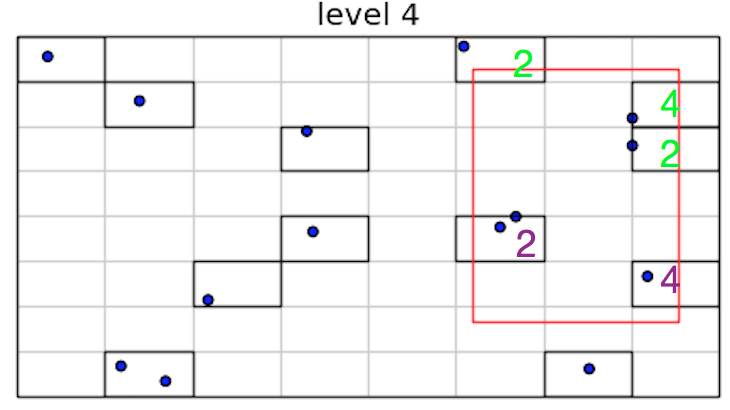
\includegraphics[width=\textwidth]{Images/2Quad_4}
  \end{minipage}
  \hfill
  \begin{minipage}[b]{0.6\textwidth}
    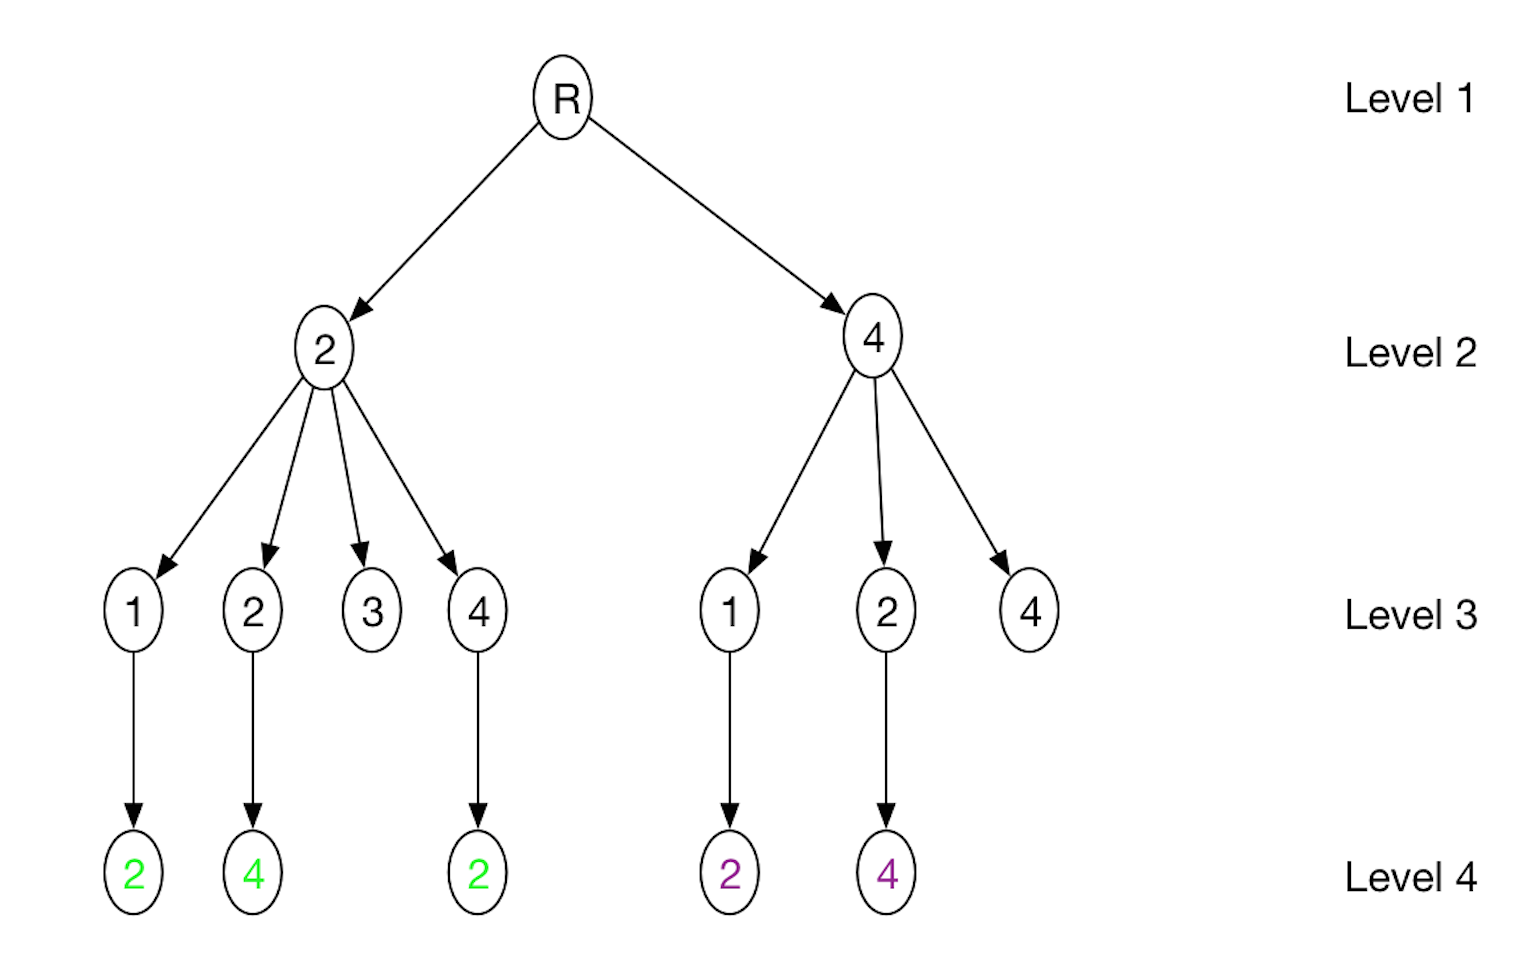
\includegraphics[width=\textwidth]{Images/2Quad_4_tree}
  \end{minipage}
  \vspace{0.5in}
  \caption{Sample Datapoints (left) and the Quadtree (right) at Level 4.}
  \label{fig:quad_2_4}
\end{figure}

\subsubsection{Query Polygon Overlapping all Leaf Nodes}

Figure~\ref{fig:quad_4_1} shows the last scenario that demonstrates a condition where the polygon contains maximum number of quadrants at level 4 of the quadtree and the algorithm provides least performance compared to all other scenarios.

\begin{figure}[H]
  \centering
  \vspace{0.5in}
  \begin{minipage}[b]{0.35\textwidth}
    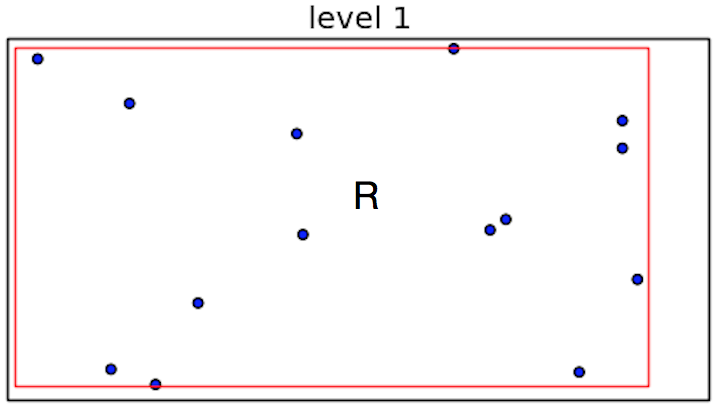
\includegraphics[width=\textwidth]{Images/4Quad1_1}
  \end{minipage}
  \hfill
  \begin{minipage}[b]{0.6\textwidth}
    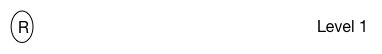
\includegraphics[width=\textwidth]{Images/1_1Quad_1_tree}
  \end{minipage}
  \vspace{0.5in}
  \caption{Sample Datapoints (left) and the Quadtree (right) at Level 1.}
  \label{fig:quad_4_1}
\end{figure}

In Figure~\ref{fig:quad_4_2} 
at level 2, the algorithm  overlaps all 4 quadrants at this level. Therefore the thread has to descend the tree from all four nodes.

\begin{figure}[H]
  \centering
  \vspace{0.5in}
  \begin{minipage}[b]{0.35\textwidth}
    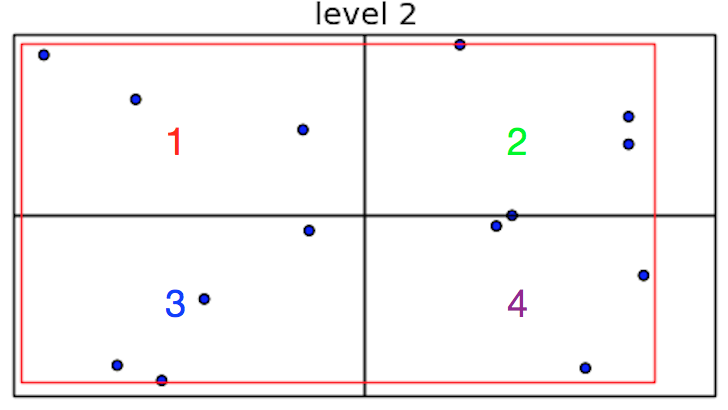
\includegraphics[width=\textwidth]{Images/4Quad1_2}
  \end{minipage}
  \hfill
  \begin{minipage}[b]{0.6\textwidth}
    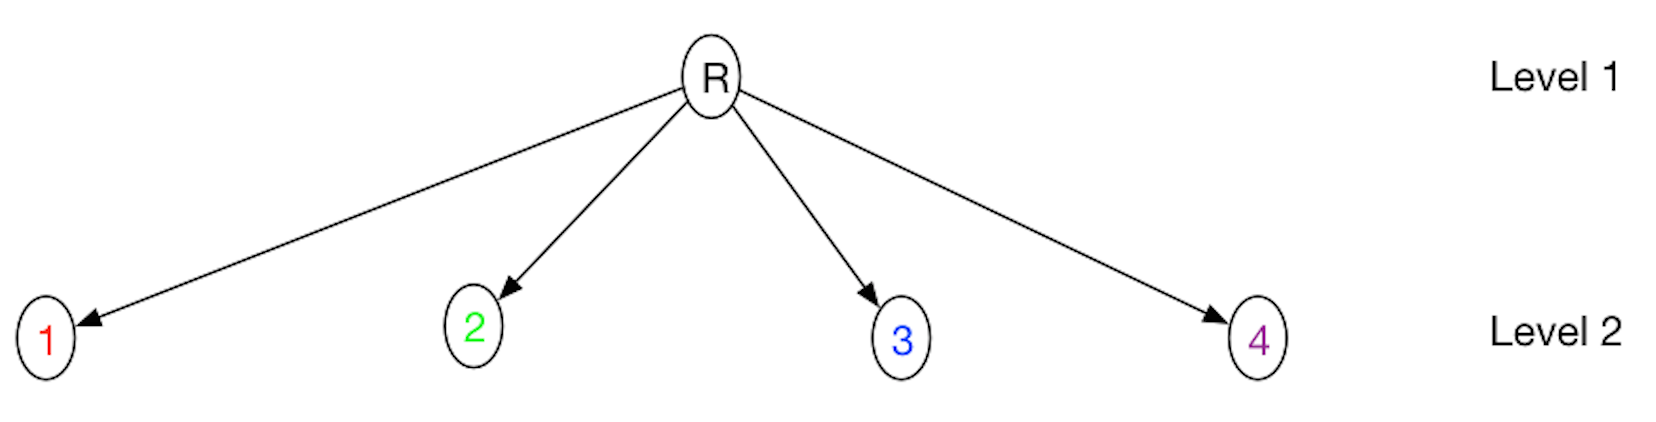
\includegraphics[width=\textwidth]{Images/1_1Quad_2_tree}
  \end{minipage}
  \vspace{0.5in}
  \caption{Sample Datapoints (left) and the Quadtree (right) at Level 2.}
  \label{fig:quad_4_2}
\end{figure}

In Figure~\ref{fig:quad_4_3} 
at level 3, the algorithm  isolates all 12 quadrants at this level. The maximum possible number of nodes at this level is 16 but four of  those nodes are empty nodes and these four nodes are ignored even though these nodes lie within the polygon.
\begin{figure}[H]
  \centering
  \vspace{0.5in}
  \begin{minipage}[b]{0.35\textwidth}
    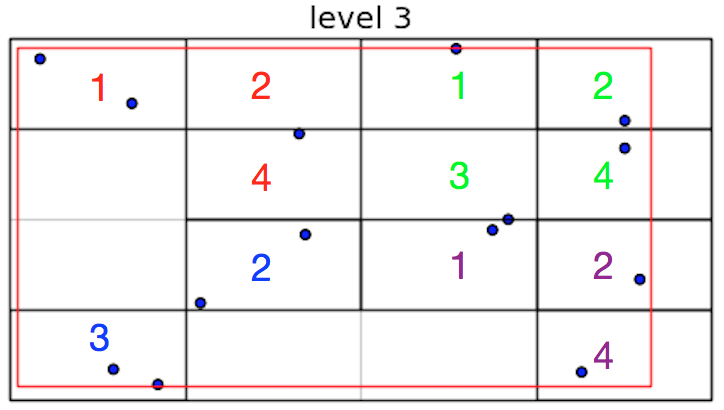
\includegraphics[width=\textwidth]{Images/4Quad1_3}
  \end{minipage}
  \hfill
  \begin{minipage}[b]{0.6\textwidth}
    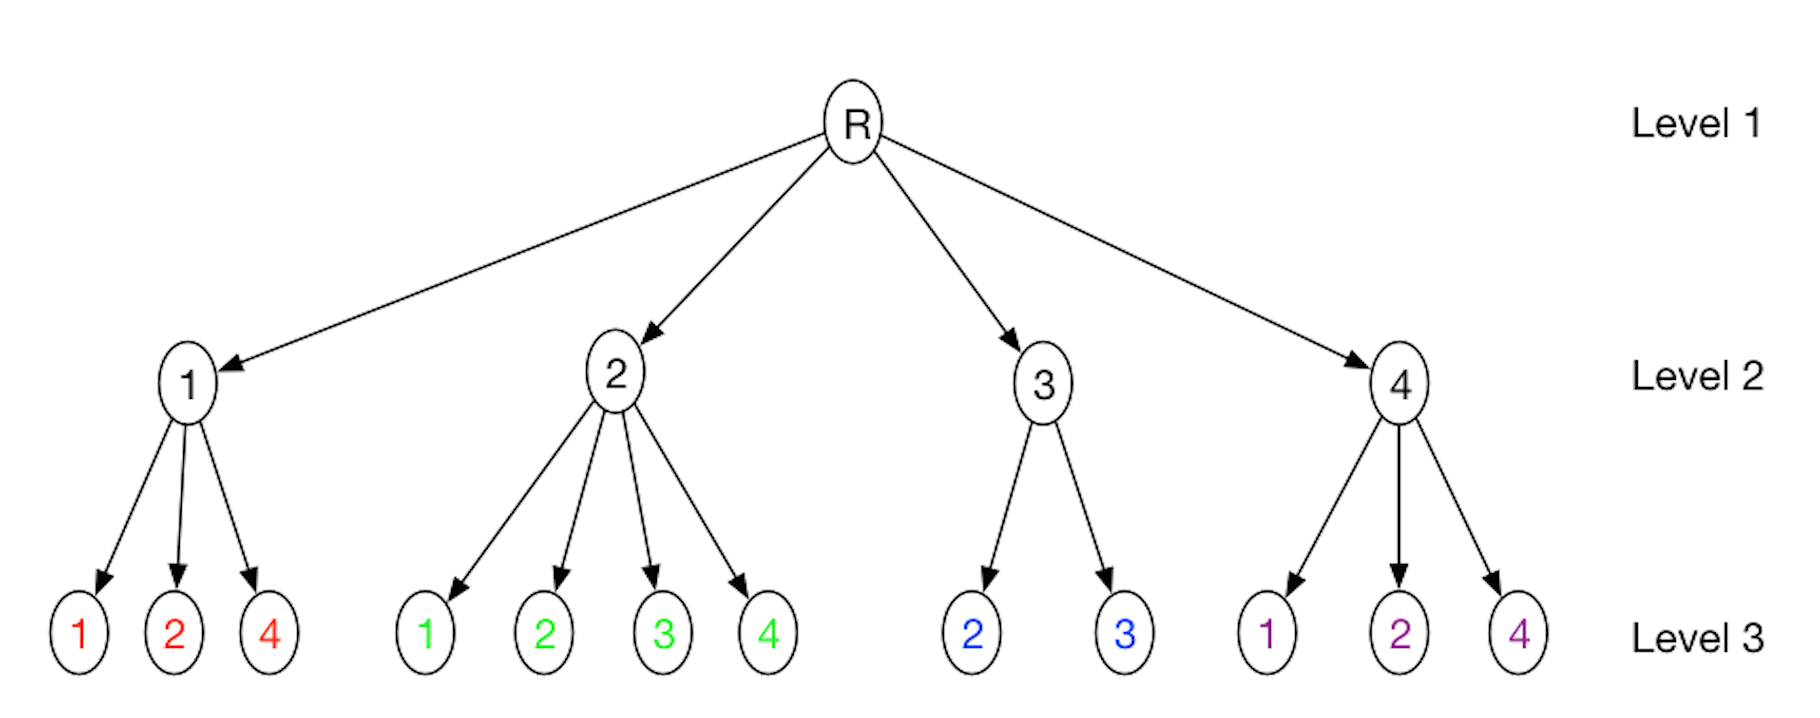
\includegraphics[width=\textwidth]{Images/1_1Quad_3_tree}
  \end{minipage}
  \vspace{0.5in}
  \caption{Sample Datapoints (left) and the Quadtree (right) at Level 3.}
  \label{fig:quad_4_3}
\end{figure}

Figure~\ref{fig:4Quad1_4} shows that at level 4, the algorithm isolates all the 12 quadrants at this level. The maximum possible number of nodes at this level is 64 but 52 of those nodes are empty nodes and  these 52 nodes are ignored even though these nodes lie within the polygon.
Finally only 12 quadrants at level 4 need to be processed in order to get the points inside the polygon in this case. If there are a larger number of data points distributed equally across the entire 2 D space and if there are no empty nodes, then all the 64 nodes need to be processed.

\begin{figure}[H]
  \centering
  \vspace{0.5in}
  \begin{minipage}[b]{0.35\textwidth}
    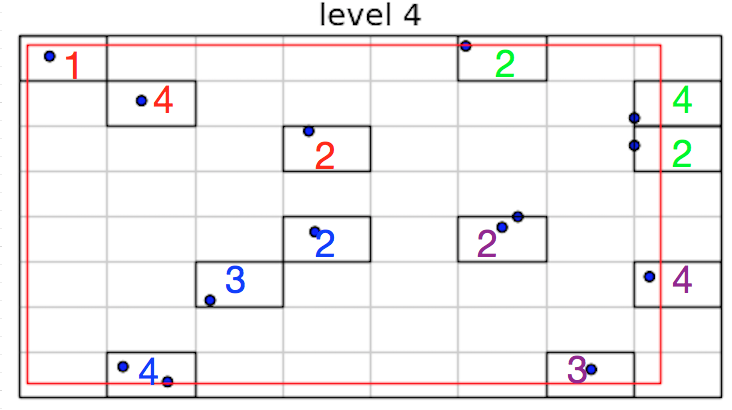
\includegraphics[width=\textwidth]{Images/4Quad1_4}
  \end{minipage}
  \hfill
  \begin{minipage}[b]{0.6\textwidth}
    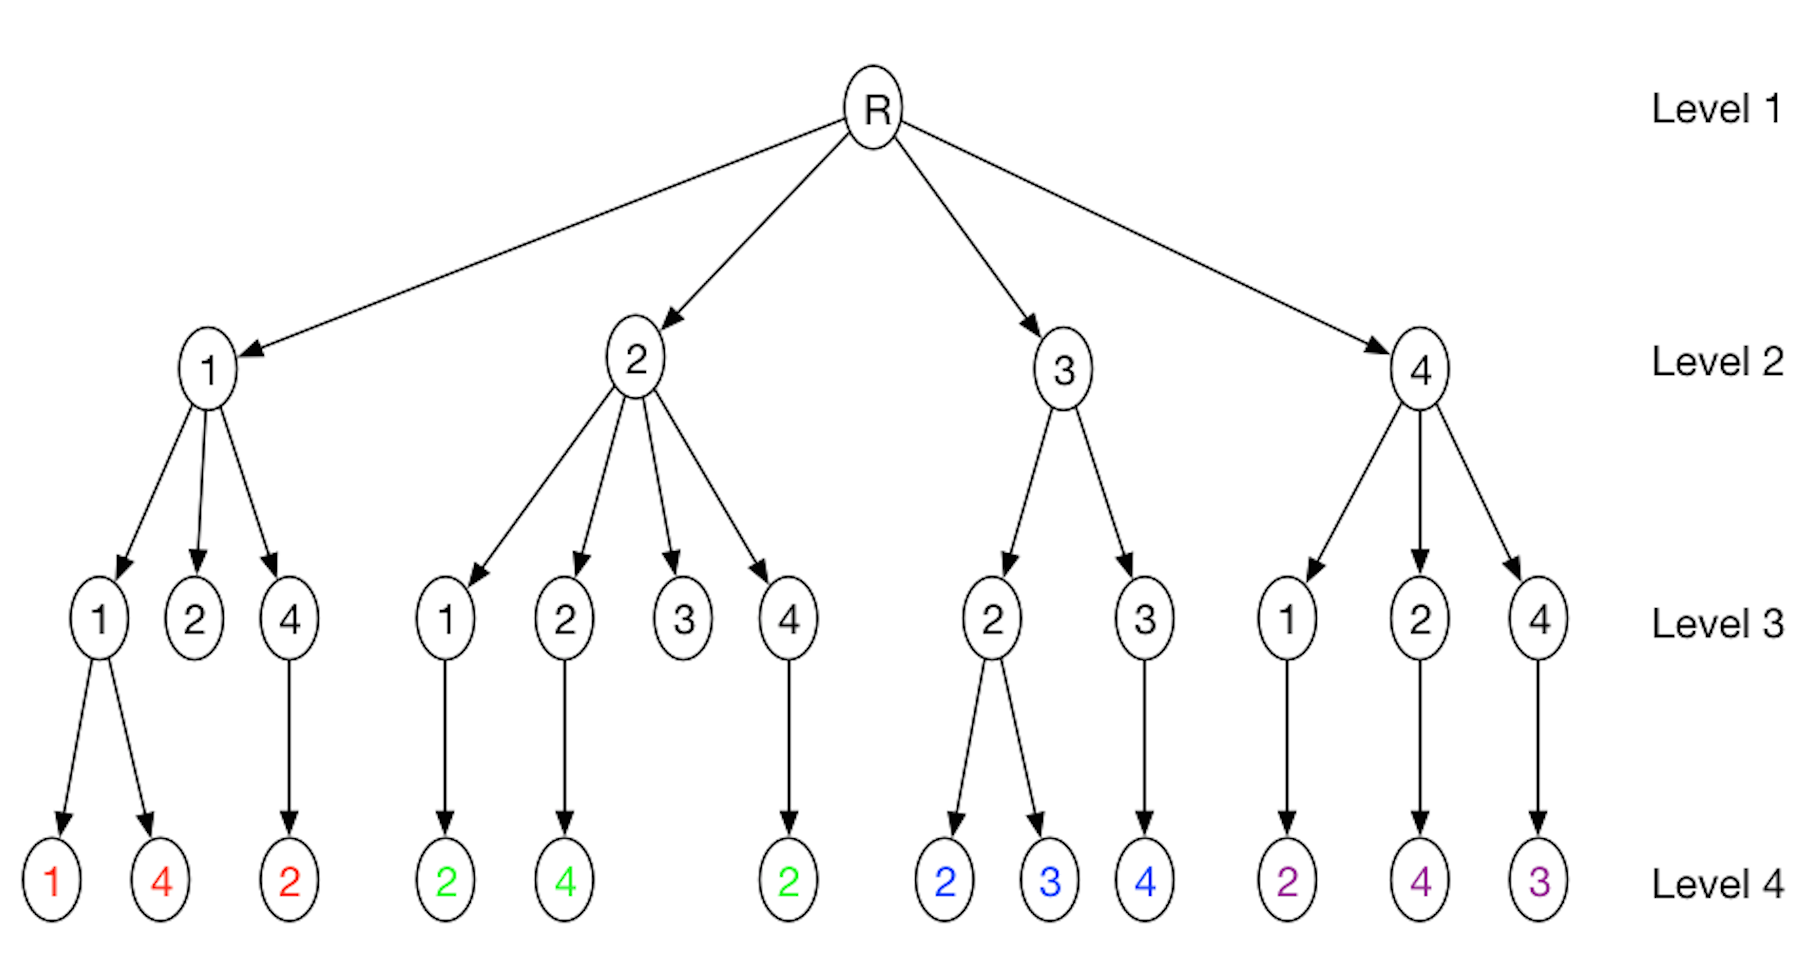
\includegraphics[width=\textwidth]{Images/1_1Quad_4_tree}
  \end{minipage}
  \vspace{0.5in}
  \caption{Sample Datapoints (left) and the Quadtree (right) at Level 4.}
  \label{fig:4Quad1_4}
\end{figure}

Figure~\ref{fig:Stack1}, shows the stack based iterative BFS traversal on GPU, in reference to Figure~\ref{fig:quad_4_3} 
and Figure~\ref{fig:4Quad1_4}. 

\begin{figure}[H]
\centering
\vspace{0.5in}
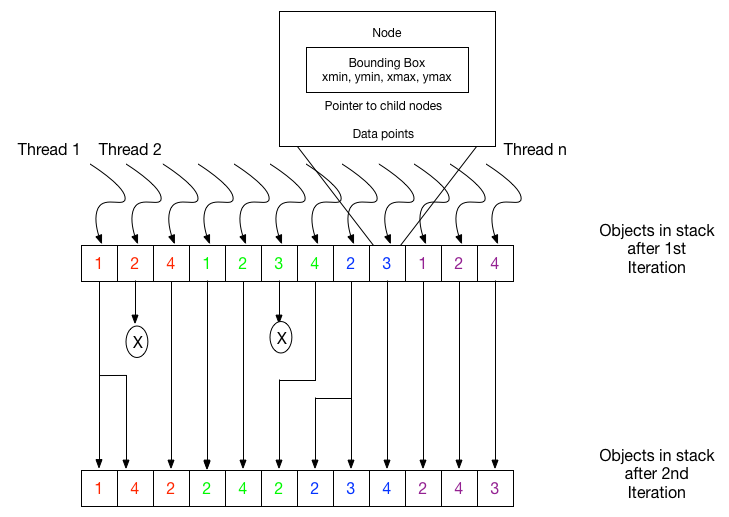
\includegraphics[scale=0.4]{Images/Stack1}
\vspace{0.5in}
\caption{Stack Based Iterative BFS Traversal.}
\label{fig:Stack1}
\end{figure}

\subsubsection{Query Polygon Containing no Points}

Figure~\ref{fig:1Quad_NoPoints} shows one case where the polygon overlaps a region where there are no points. 

\begin{figure}[ht]
  \centering
  \vspace{0.5in}
  \begin{minipage}[b]{0.35\textwidth}
    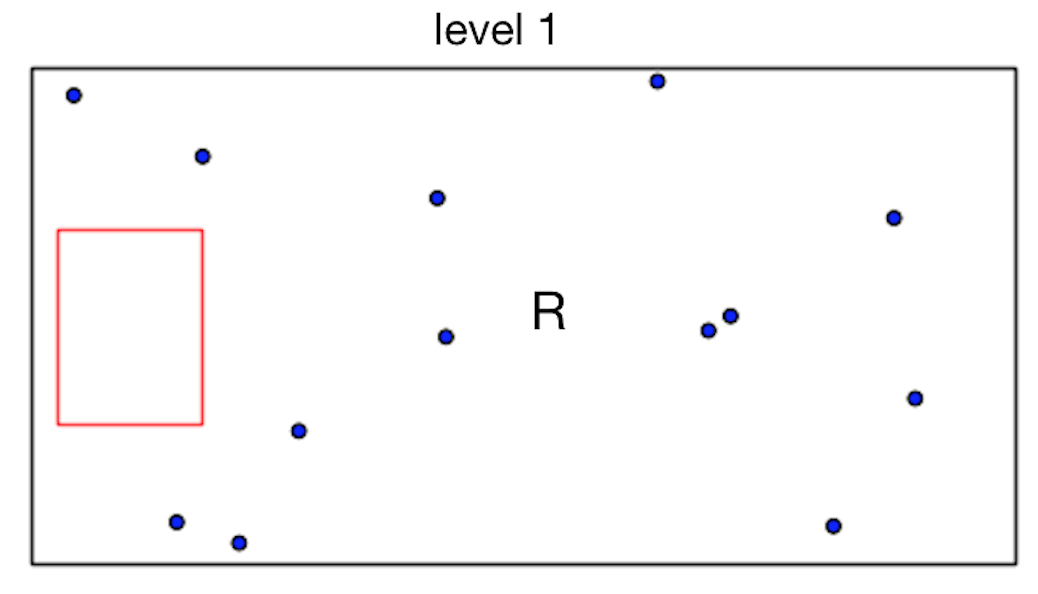
\includegraphics[width=\textwidth]{Images/NoPointQuad1}
  \end{minipage}
  \hfill
  \begin{minipage}[b]{0.6\textwidth}
    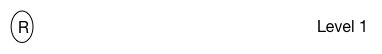
\includegraphics[width=\textwidth]{Images/1_1Quad_1_tree}
  \end{minipage}
  \vspace{0.5in}
  \caption{Sample Datapoints (left) and the Quadtree (right) at Level 1.}
  \label{fig:1Quad_NoPoints}
\end{figure}

Figure~\ref{fig:2Quad_NoPoints} shows two distinct cases. At level 2, the algorithm isolates first and third child of the root node.
At level 3, the polygon does not overlap with any of the children of the nodes from level 2. The nodes that it overlaps are empty nodes and therefore the tree is not traversed any further.

\begin{figure}[ht]
  \centering
  \vspace{0.5in}
  \begin{minipage}[b]{0.35\textwidth}
    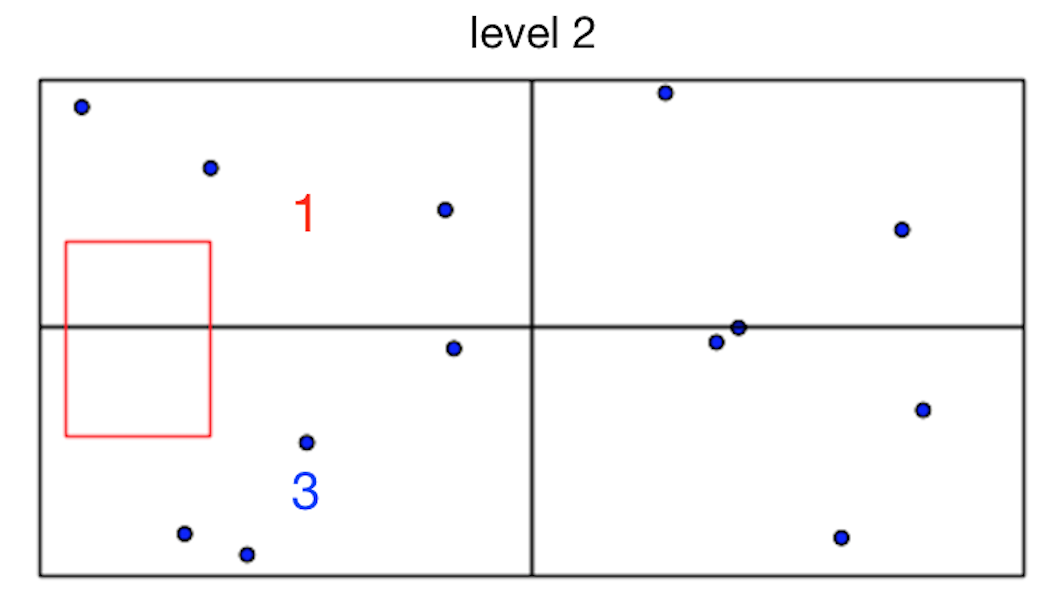
\includegraphics[width=\textwidth]{Images/NoPointQuad2}
  \end{minipage}
  \hfill
  \begin{minipage}[b]{0.6\textwidth}
    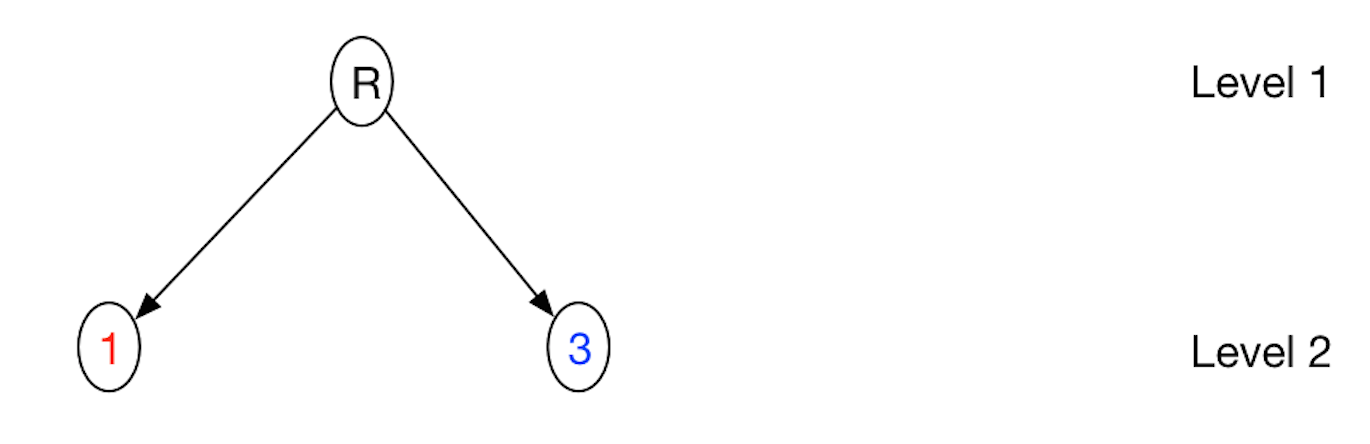
\includegraphics[width=\textwidth]{Images/NoPoints3_1}
  \end{minipage}
  \vspace{0.5in}
  \caption{Sample Datapoints (left) and Quadtree (right) at Level 2.}
  \label{fig:2Quad_NoPoints}
\end{figure}



